\documentclass[11pt,letterpaper]{article}

\usepackage{fontspec}
\usepackage[utf8]{inputenc}
\usepackage{textcomp,marvosym}
\usepackage{amsmath,amssymb}
\usepackage[left]{lineno}
\usepackage{changepage}
% rotating package for sideways tables
\usepackage{rotating}
\usepackage{natbib}
\usepackage{setspace} 
\doublespacing

\raggedright
\textwidth = 6.5 in
\textheight = 8.5 in
\oddsidemargin = 0.0 in
\evensidemargin = 0.0 in
\topmargin = 0.0 in
\headheight = 0.0 in
\headsep = 0.5 in
\parskip = 0.1 in
\parindent = 0.1in

% Bold the 'Figure #' in the caption and separate it from the title/caption with a period
% Captions will be left justified
\usepackage[aboveskip=1pt,labelfont=bf,labelsep=period,justification=raggedright,singlelinecheck=off]{caption}

% Remove brackets from numbering in List of References
\makeatletter
\renewcommand{\@biblabel}[1]{\quad#1.}
\makeatother

% Leave date blank
\date{}

% Header and Footer with logo
\usepackage{lastpage,fancyhdr,graphicx}
\usepackage{epstopdf}
\pagestyle{myheadings}
\pagestyle{fancy}
\fancyhf{}
\lhead{Swanson-Hysell et al. (2015) Paleomagnetic pole for the Umkondo LIP}
\rhead{\thepage/\pageref{LastPage}}
%\renewcommand{\footrule}{\hrule height 2pt \vspace{2mm}}
%\fancyheadoffset[L]{2.25in}
%\fancyfootoffset[L]{2.25in}
%\lfoot{\sf }

%% END MACROS SECTION

\begin{document}

\begin{flushleft}
{\Large \textbf{A new grand mean paleomagnetic pole for the 1.11 Ga Umkondo Large Igneous Province with implications for paleogeography and the geomagnetic field}}
\\
N.L. Swanson-Hysell\textsuperscript{1,*},
T.M. Kilian\textsuperscript{1},
R.E. Hanson\textsuperscript{2}
\\
\bigskip
\textsuperscript{1} Department of Earth and Planetary Science, University of California, Berkeley, CA 94720, USA
\\
\textsuperscript{2} School of Geology, Energy, and the Environment, Texas Christian University, Fort Worth, TX 76129, USA
\\
\bigskip
* swanson-hysell@berkeley.edu

The citation for this work is:

Swanson-Hysell, N.L., Kilian, T.M., and Hanson, R.E., 2015, A new grand mean paleomagnetic pole for the 1.11 Ga Umkondo Large Igneous Province with implications for paleogeography and the geomagnetic field, \textit{Geophysical Journal International}, doi:10.1093/gji/ggv402.

\end{flushleft}

\linenumbers

\section*{Summary}
We present a new grand mean paleomagnetic pole (Plong: 222.1\textdegree, Plat: -64.0\textdegree, A$_{95}$: 2.6\textdegree, N=49) for the ca. 1110 Ma Umkondo Large Igneous Province (LIP) of the Kalahari Craton. New paleomagnetic data from 24 sills in Botswana and compiled reprocessed existing data are used to develop a paleomagnetic pole as the Fisher mean of cooling unit virtual geomagnetic poles (VGPs). The mean and its associated uncertainty provide the best-constrained pole yet developed for the province. Comparing data from individual cooling units allows for evaluation of paleosecular variation at this time in the Mesoproterozoic. The elongation of the population of VGPs is consistent with that predicted by the TK03.GAD model lending support to the dipolar nature of the field in the late Mesoproterozoic. In our new compilation, 4 of 59 ($\sim$7$\%$) of the igneous units have northerly declinations while the rest are south-directed indicating that a geomagnetic reversal occurred during magmatic activity. Interpreting which of these polarities corresponds with a normal or reversed geomagnetic field relative to other continents can constrain the relative orientations between cratons with time-equivalent data. This interpretation is particularly important in comparison to Laurentia as it bears on Kalahari's involvement and position in the supercontinent Rodinia. The dominance of south-directed declinations within the Umkondo Province was previously used to suggest that these directions are the same polarity as reversed directions from the early magmatic stage of the Keweenawan Midcontinent Rift of Laurentia. Two Umkondo sills with northerly declinations have U-Pb baddeleyite ages of ca. 1109 Ma that are temporally close to dated Midcontinent rift units having reversed directions. Based on this comparison, and paleomagnetic data from younger units in the Kalahari Craton, we favor the option in which the sites with northerly declinations from the Umkondo Province correspond to the reversed polarity directions from the early magmatic stage in the Midcontinent Rift. This interpretation allows for the Namaqua-Natal metamorphic belt of Kalahari to be a conjugate to the Grenville margin of North America and for Kalahari to have become conjoined with Laurentia within the supercontinent Rodinia subsequent to Umkondo LIP magmatic activity.

\section*{Introduction}
Paired paleomagnetic and geochronologic data demonstrate that between ca. 1112 and 1108 Ma there was large-scale magmatism across the Kalahari Craton over an area of $\sim$2 x 10$^6$ km$^2$ (Fig. \ref{fig:map}; \citealp{Hanson2004a}). Extrusive components of this province are exposed as tholeiitic basalts that occur at the top of the Umkondo Group in Zimbabwe and Mozambique \citep{Swift1962a, McElhinny1966a, Moabi2015a} and as rhyolite lavas, pyroclastics and tholeiitic basalts within the Kgwebe Formation of northern Botswana \citep{Modie1996a, Hanson2006a}. However, the majority of exposed remnants of the Umkondo Large Igneous Province (LIP) are shallow-level mafic intrusions \citep{Hanson2006a, Kock2014a} which are interpreted as feeders to more extensive flood lavas that have largely eroded away \citep{Hanson2004a}.

\begin{figure}[h!]
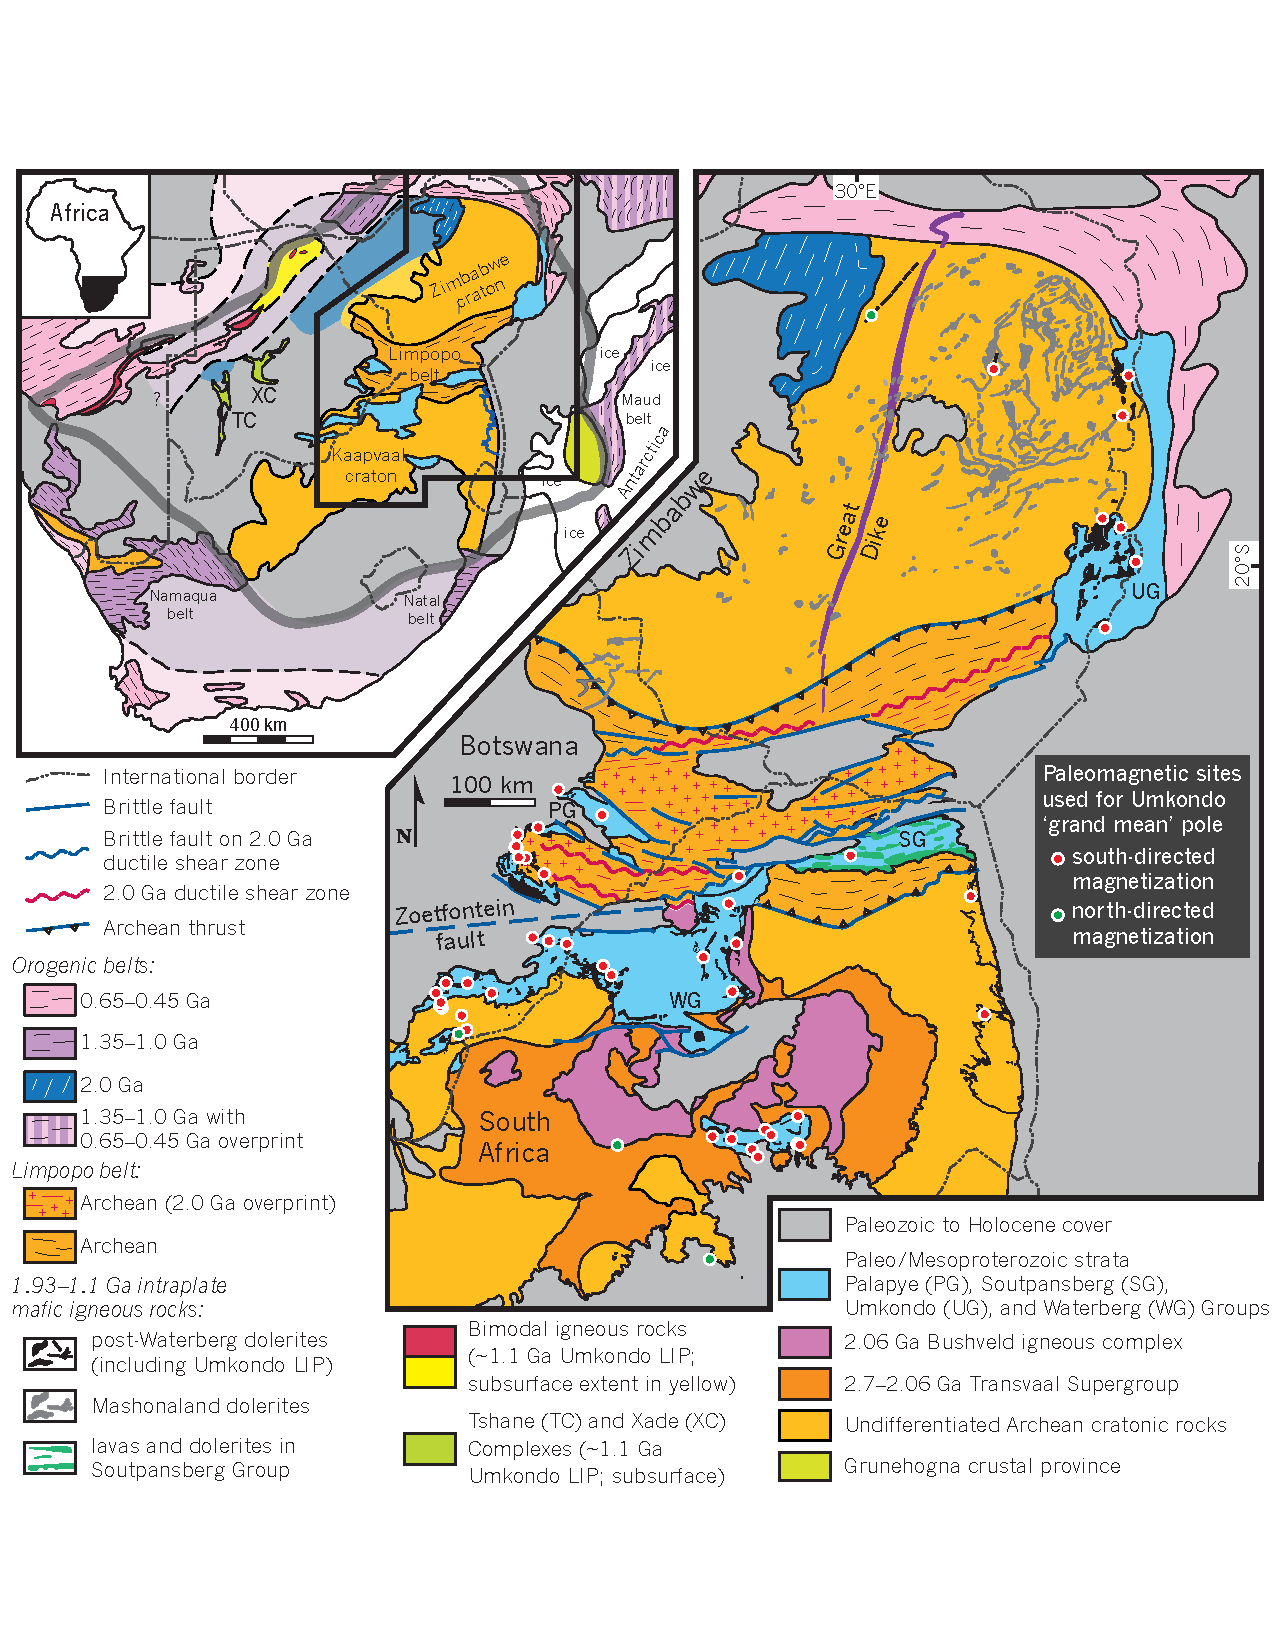
\includegraphics[width=5.7 in]{figures/Umkondo_locality_map.pdf}
\caption{\textbf{ Geological map modified from \cite{Hanson2011b} showing locations of paleomagnetic sites (individual cooling units) in the ca. 1110 Ma Umkondo LIP used in this study.} See \cite{Hanson2011b} for sources for the geological data. The inset map shows the location of the main map and the broader geological context. The thick translucent gray line on the inset map indicates the interpreted shape of the Kalahari Craton on the interior of the late Mesoproterozoic orogenic belts that is used in the paleogeographic reconstructions (Fig. \ref{fig:reconstruction}). Remnants of the Umkondo LIP are preserved across the Kalahari Craton including: intrusions and lavas in the Grunehogna crustal province of Antarctica (rotated to Kalahari), the abundant dolerite sills throughout South Africa and Botswana, the Umkondo lavas of Zimbabwe and Mozambique, the subsurface Tshane and Xade Complexes of central Botswana and the bimodal igneous rocks of the Kgwebe Formation in the far northwest portion of the craton.}
\label{fig:map}
\end{figure}

The widespread extent of these intrusions has led to the inference that the lavas covered nearly all of the Kalahari Craton. In many areas in the craton where pre-1.1 Ga rocks are exposed, known Umkondo intrusions occur together with Paleoproterozoic mafic intrusions and intrusions related to the 183 Ma Karoo LIP \citep{Svensen2012a}. In the absence of petrophysical, geochronological or paleomagnetic constraints, it may be difficult to distinguish units belonging to these different intrusive suites.

Paleomagnetic data from Umkondo intrusions have been used to develop a ca. 1110 Ma paleomagnetic pole that is a crucial constraint on Kalahari's paleogeographic position at that time \citep{Powell2001a,Gose2006a}. This pole demonstrates that, despite the similar ages of magmatic activity in the Umkondo LIP and magmatism associated with the initiation of the Keweenawan Midcontinent Rift in Laurentia, Kalahari and Laurentia were separated by $>$30\textdegree\ of latitude at the time. Kalahari is hypothesized to have become conjoined with other continents in the supercontinent Rodinia subsequent to Umkondo magmatic activity \citep{Jacobs2008a,Li2008a}. High-grade metamorphic rocks in the Namaqua-Natal-Maud belt are interpreted to be a record of ca. 1090 to 1060 Ma orogenesis associated with continent-continent collision \citep{Jacobs2008a}. 

\section*{Umkondo Sills in Botswana}
In southeastern Botswana, abundant mafic sills and sheets intrude Paleoproterozoic sedimentary rocks and underlying Archean basement rocks.  Single-crystal U-Pb baddeleyite crystallization ages have been obtained for six of these Botswana intrusions and indicate that five of them correspond to the time period of Umkondo LIP emplacement \citep{Hanson2004a}. In addition to these five dated Umkondo examples, an additional five intrusions in Botswana have previously been shown to correspond to the Umkondo LIP due to the close correspondence of their paleomagnetic directions to the mean for the Umkondo LIP (\citealp{Jones1966a}, \citealp{Gose2006a}; Table 1). In many cases, single intrusions have been sampled for paleomagnetism at multiple sites. For example, there are nine published sites within the Shoshong Sill (six from \cite{Jones1966a} and three from \cite{Gose2006a}). Dates from dolerite sills and other intrusions in Zimbabwe and South Africa are similar in age to those from Botswana indicating that there was a craton-scale magmatic event between ca. 1112 and 1108 Ma \citep{Hanson2004a}.

In the vicinity of Shoshong, the sills have been referred to as the Dibete-Shoshong differentiated suite \citep{Carney1994a} and dominantly intrude the Paleoproterozoic sediments of the Palapye Group, although they were emplaced into the Paleoproterozoic Mahalapye and Mokgware Granites as well. Further south, near Molepolole, sills of the Kanye-Mochudi dolerite suite primarily intrude Paleoproterozoic sediments of the Waterberg Group, with some of the units in the southern part of the study area intruding the Archean Gaborone Granite \citep{Carney1994a}. All of these high-level mafic intrusions have generally been grouped together as ``post-Waterberg'' dolerites, and we therefore use the prefix ``PW'' when referring to our sample localities in the region. Where reliable paleomagnetic or geochronological data are lacking, the dolerites are broadly constrained by geological relations to be younger than the Waterberg Group and older than the Carboniferous-Jurassic Karoo Supergroup. 

Although there are many sills in southeastern Botswana without geochronological or paleomagnetic data, it is assumed that the vast majority of these sills correspond to the Umkondo LIP (e.g., Fig. 9 of \citealp{Hanson2006a}). This assumption, while shown to be true in this study, is complicated by the spatial overlap of the Umkondo Province with other dolerite intrusions with a range in U-Pb isotopic ages. These include the 1.93 Ga Moshaneng dolerites in Botswana \citep{Hanson2004b}, the 1.88-1.87 Ga Mashonaland Igneous Province in Zimbabwe and coeval dolerites intruding the Waterberg Group in South Africa \citep{Hanson2004b,Hanson2011b,Soderlund2010a}, post-1.83 Ga dolerite sills in the Soutpansberg Group \citep{Brandl1981a,Brandl1985a,Geng2014a}, and the widespread 0.18 Ga Karoo LIP \citep{Sell2014a}. It is a testament to the mild post-2.0 Ga metamorphic history of the interior of the Kalahari Craton that dolerites dated at ca. 1.9 Ga, 1.1 Ga and 0.2 Ga all have similar appearance in the field. While the interpretation that the bulk of dolerite intrusions within the Waterberg and Palapye groups and the underlying basement correspond to the Umkondo event is a reasonable one, it is largely untested since there are precise age constraints for only a small fraction of the total exposed intrusions. If high-quality paleomagnetic data can be generated from a given sill, the distinct paleomagnetic poles from ca. 1.9 Ga, Umkondo and Karoo dolerites provide a means of discriminating mafic intrusions belonging to these intraplate igneous provinces. Through this work, we can now show with a combination of paleomagnetic and geochronologic data that 25 intrusions from southeastern Botswana are associated with Umkondo magmatism.

\section*{Methods and results}

Samples were collected in the field in southeastern Botswana with a gas-powered drill and oriented using a Pomeroy orienting device. Given that large local deviations in magnetic declination occur locally in association with rock struck by lightning, sun compass data were used exclusively for determining the declination of oriented core samples. The sundec.py program of the PmagPy software package (https://github.com/ltauxe/PmagPy) was used for sun compass calculations.

\begin{figure}[h!]
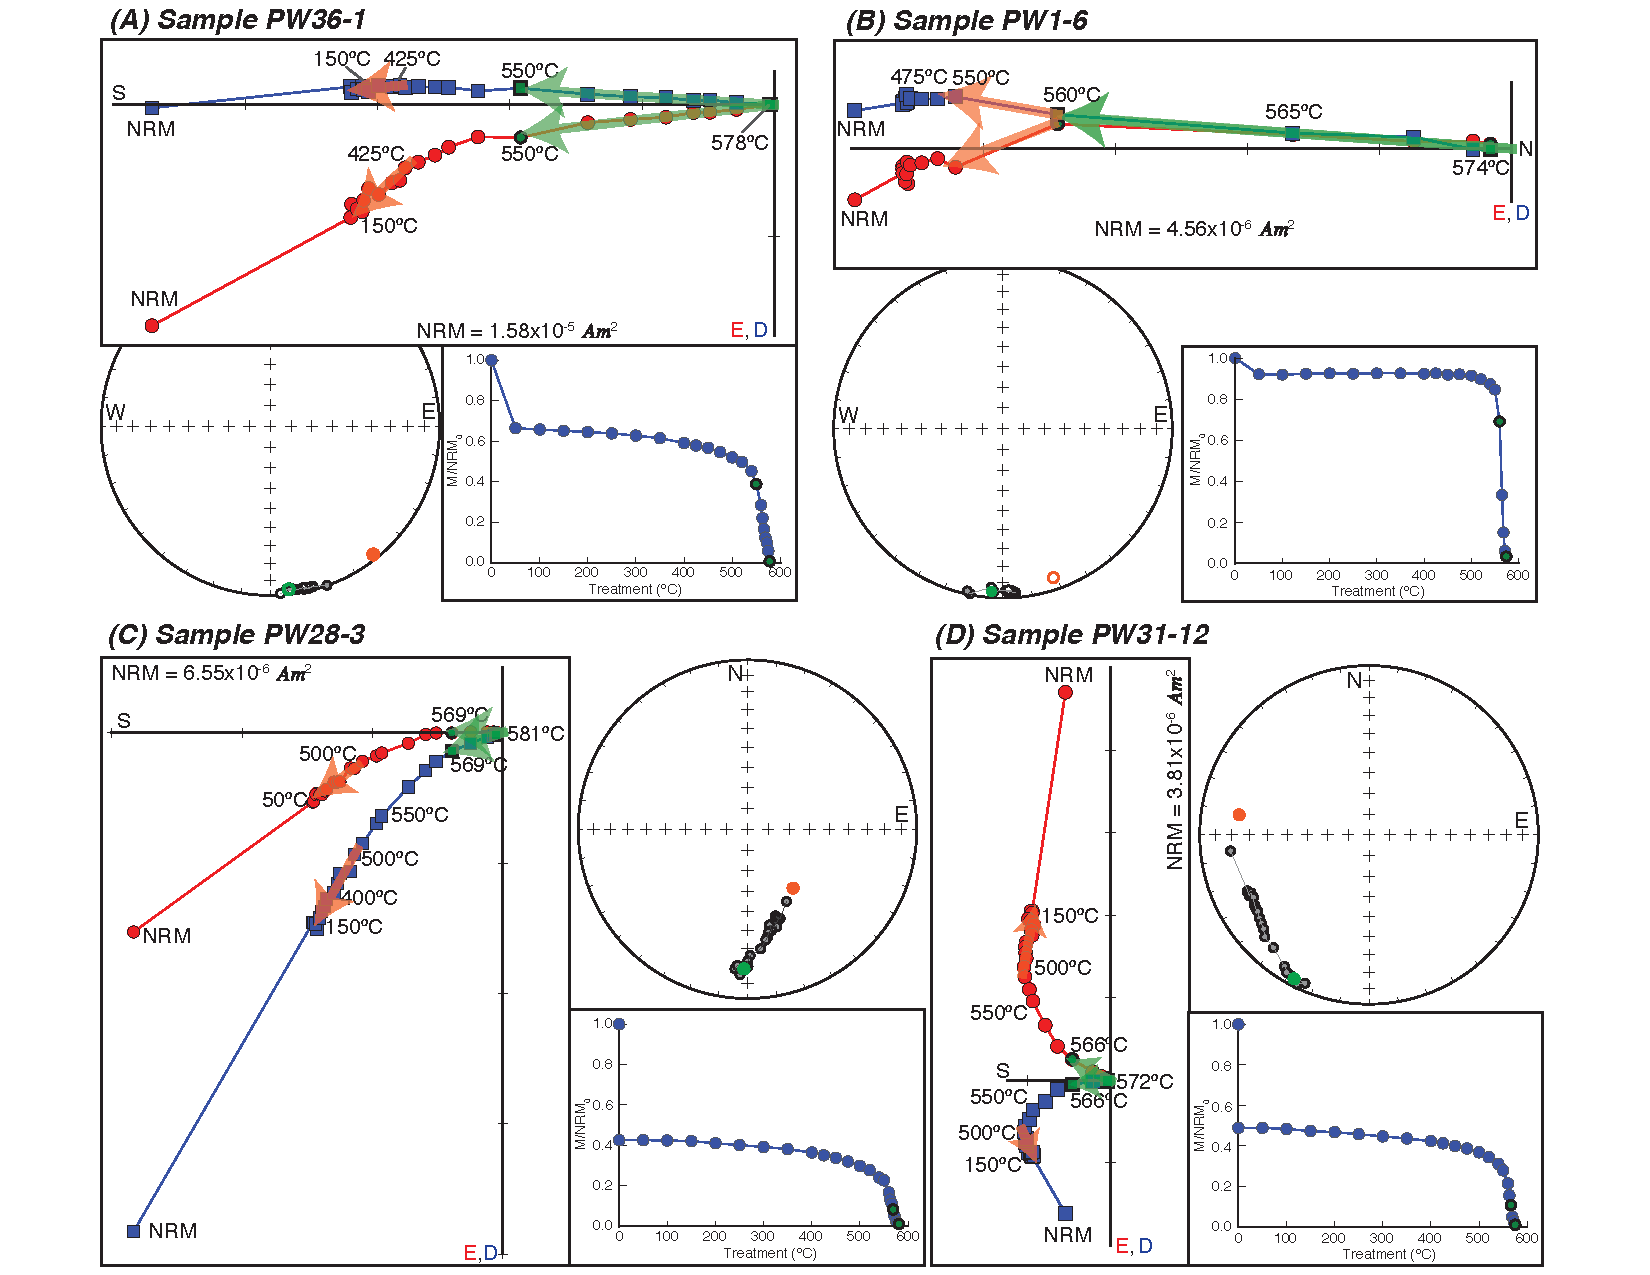
\includegraphics[width=6.5 in]{figures/Umkondo_pmag_data.pdf}
\caption{\textbf{ Example paleomagnetic data from Umkondo dolerite sills in southeastern Botswana.} Thermal demagnetization data shown in vector component diagrams, equal-area plots and normalized intensity vs. temperature plots for four samples from four Umkondo sills. Least-squares fits are shown on both the vector component diagrams and equal-area plots for the low-temperature (orange) and high-temperature (green) portions of the demagnetization data.}
\label{fig:pmag}
\end{figure}

Samples from every site underwent alternating field (AF) demagnetization at the Institute for Rock Magnetism (IRM) at the University of Minnesota using a 2G Enterprises DC-SQUID superconducting rock magnetometer (Fig. \ref{fig:pmag}). A subset of samples from 31 out of 40 sampled localities was selected for thermal demagnetization at the UC Berkeley Paleomagnetism Lab using a 2G Enterprises DC-SQUID superconducting rock magnetometer. Both magnetometers are housed in large magnetostatic shields with magnetic fields $<$500 nT. The quartz glass sample rod of the UC Berkeley system is typically measured at 5 x 10$^{-12}$ Am$^2$ and the mylar track and sample holders on the IRM system are typically measured between 5 x 10$^{-11}$ and 2 x 10$^{-10}$ Am$^2$. After measurement of the natural remanent magnetization (NRM), and prior to thermal and AF demagnetization steps, the samples underwent liquid nitrogen immersion in a low-field environment ($<$10 nT). This step was implemented with the goal of preferentially removing remanence associated with multidomain magnetite. Such multidomain grains undergo low-temperature demagnetization when cycled through the isotropic point ($\sim$130 K) and the Verwey transition ($\sim$120 K; \cite{Verwey1939a, Feinberg2015a}). The overprints removed during this low-temperature demagnetization step were in some cases quite large (Fig. \ref{fig:pmag}) and the associated progressive loss of remanence was explored in detail for two of the Botswana dolerite samples in a study by \cite{Feinberg2015a}. Following acquisition of the data, principal component analysis \citep{Kirschvink1980a} was conducted using the PmagPy software package (https://github.com/ltauxe/PmagPy).

Magnetic vectors removed through progressive demagnetization and interpreted as overprints were not well-grouped (see Supporting Information) suggesting that lightning remagnetization may be a dominant process due to the low rates of landscape evolution and denudation in the region. Of 32 studied sills, 27 yielded coherent groupings of directions that we interpret as primary thermal remanent magnetizations. Of these sills, we interpret 24 to correspond to the Umkondo LIP (Table 1; details in the Supporting Information). An additional sill in the Mokgware Hills area has been dated to be of Umkondo age (1109.2 $\pm$ 0.5 Ma; sample JP29 of \cite{Hanson2004a}), but yielded scattered paleomagnetic data in the study of \cite{Pancake2001a} and was not resampled for this study.

Throughout southeastern Botswana, the dolerite sills and sheets are predominantly sub-horizontal with dips less than 10\textdegree. We apply a tilt correction to sites where the tilt of the intrusions could be inferred either through the orientation of the tabular body itself or through the orientation of adjacent host sedimentary strata. These corrections are detailed within the Supporting Information and are applied to the tilt-corrected directions reported in Table 1.

\begin{table}[!ht]
\begin{adjustwidth}{-0.0in}{0in}
\begin{tiny}
\caption{
\textbf{Umkondo LIP paleomagnetic data by site (cooling unit)}}
\begin{tabular}{p{2.0 cm}p{1.25 cm}llllllllllll}
\hline
Site & Locales &  Site &  Site  &  n  & Dec  &  Inc & Dec$_{TC}$ & Inc$_{TC}$ & $\alpha_{95}$ & k & Date &  VGP &  VGP \\

name & used &  lat (\textdegree N) &  long (\textdegree E) &     &  (\textdegree) &  (\textdegree) &  (\textdegree)
& (\textdegree) &  &  & (Ma) &  lat (\textdegree N) &  long (\textdegree E) \\

\hline
Kgale Peak Sill          &                   PW1 and PW2 &   -24.688 &     25.862 &   12 &  189.7 &   5.3 &   189.9 &     0.4 &   6.3 &   48.8 &  1108.0 $\pm$ 0.9 &     -63.7 &      228.7 \\
Rasemong Sill            &                              PW5 &   -24.727 &     25.776 &    8 &   14.4 & -18.6 &    14.4 &   -18.6 &   8.1 &   48.0 &      &      69.6 &       70.4 \\
Metsemotlhaba River Sill &                              PW6 &   -24.547 &     25.809 &    7 &  180.6 &  -2.7 &   180.6 &    -2.7 &  14.4 &   18.5 &      &     -64.1 &      207.2 \\
Mabogoapitse Hill Sill   &                   PW7 and PW8 &   -24.474 &     25.597 &    9 &  184.6 &   5.1 &   184.6 &     5.1 &   9.1 &   33.2 &      &     -67.6 &      217.8 \\
Semarule Hill Sill       &                              PW9 &   -24.453 &     25.574 &    5 &  186.8 &   3.8 &   186.8 &     3.8 &   9.1 &   72.2 &      &     -66.5 &      222.8 \\
Rapitsane Sill           &                             PW10 &   -24.420 &     25.585 &    8 &  197.9 &  -4.9 &   197.7 &    -0.2 &   8.5 &   43.3 &      &     -60.1 &      243.1 \\
Suping Sill              &                    PW11 and JP15 &   -24.328 &     25.532 &   16 &  188.9 &  -9.8 &   187.2 &    -9.2 &   8.4 &   20.2 &      &     -60.2 &      220.1 \\
Mogatelwane 2 Sill       &                             PW15 &   -24.180 &     25.692 &    6 &  193.6 &  -1.2 &   193.5 &    -2.8 &  14.7 &   21.6 &      &     -61.3 &      234.7 \\
Mosolotsane 1 Sill       &  PW21, PW22, and JP(22,23,24) &   -22.907 &     26.389 &   27 &  186.9 &  -3.2 &   186.1 &    -5.6 &   4.6 &   36.9 &  1109.3  $\pm$ 0.6 &     -63.6 &      220.2 \\
Mosolotsane 5 Sill       &                             PW23 &   -22.903 &     26.370 &    7 &  189.6 &  -5.1 &   188.5 &    -7.9 &  14.2 &   19.1 &      &     -61.9 &      224.6 \\
Mosolotsane 4 Sill       &                              PW24 &   -22.895 &     26.374 &    8 &  185.4 &  -0.3 &   185.2 &    -2.5 &   7.9 &   50.3 &      &     -65.3 &      218.9 \\
Mosolotsane 6 Sill       &                              PW25 &   -22.896 &     26.367 &    5 &  188.9 &  14.8 &   191.2 &    11.8 &   9.0 &   72.7 &      &     -69.9 &      240.6 \\
Mosolotsane 3 Sill       &                              PW26 &   -22.893 &     26.381 &    4 &  189.7 &   2.0 &   189.8 &    -0.9 &  16.7 &   31.3 &      &     -64.8 &      229.9 \\
Mosolotsane 2 Sill       &                              PW27 &   -22.892 &     26.382 &    8 &  187.0 &   4.5 &   187.6 &     2.0 &   5.6 &   97.5 &      &     -66.9 &      226.1 \\
Shoshong Sill            &          PW28 and JP(26,31,33,34) &   -23.005 &     26.484 &   33 &  191.5 &  -5.4 &   191.5 &    -5.4 &   3.1 &   65.2 &  1109.3  $\pm$ 0.4 &     -61.9 &      231.5 \\
Phage Sill               &                              PW29 &   -22.779 &     26.394 &    8 &  193.9 &   1.6 &   194.0 &    -0.8 &   7.8 &   50.9 &      &     -63.1 &      238.7 \\
Moijabana Sill           &                              PW30 &   -22.642 &     26.443 &    5 &  189.4 & -10.0 &   189.4 &   -10.0 &  17.9 &   19.2 &      &     -60.8 &      225.9 \\
Mokgware Sill            &                    PW31 and JP30 &   -22.707 &     26.611 &   13 &  199.2 &   2.5 &   199.0 &     3.8 &   6.5 &   42.2 &  1112.0  $\pm$ 0.5 &     -62.2 &      250.8 \\
Sepatamorire Sill        &                             PW32 &   -22.335 &     26.823 &    8 &  194.1 &   1.5 &   194.1 &     1.5 &   8.3 &   45.6 &      &     -64.4 &      241.2 \\
Palapye dike             &                              PW33 &   -22.578 &     27.287 &    7 &  172.5 &   7.1 &   173.6 &    13.9 &  11.4 &   29.0 &      &     -73.3 &      184.6 \\
Masama 1 Sill            &                             PW34 &   -23.816 &     26.738 &    8 &  169.6 & -21.1 &   170.5 &   -13.6 &   8.8 &   40.3 &      &     -57.9 &      188.8 \\
Masama 3 Sill            &                 PW35 and PW37 &   -23.814 &     26.735 &   13 &  188.5 &  -8.7 &   188.5 &    -0.7 &   4.8 &   75.4 &      &     -64.5 &      226.8 \\
Masama 2 Sill            &                             PW36 &   -23.815 &     26.735 &    8 &  183.2 &  -4.4 &   183.2 &     3.5 &   7.7 &   53.1 &      &     -67.7 &      215.2 \\
Dibete Kop Sill          &                             PW38 &   -23.782 &     26.563 &    7 &  194.4 &   0.8 &   194.4 &     0.8 &   9.4 &   42.4 &      &     -62.8 &      239.5 \\
W01-W02                  &                              W01-W02 &   -25.480 &     29.450 &   25 &     &    &   175.6 &   -18.4 &   6.2 &   22.6 &      &     -54.8 &      201.9 \\
W04                      &                                  W04 &   -25.750 &     29.450 &   12 &     &    &   171.5 &   -22.3 &   4.9 &   80.8 &      &     -51.8 &      195.9 \\
W05                      &                                  W05 &   -25.760 &     29.480 &   11 &     &    &   176.4 &    -7.8 &   7.5 &   38.0 &      &     -60.1 &      202.3 \\
W08-W09                  &                              W08-W09 &   -25.620 &     29.100 &   20 &     &    &   192.8 &    15.9 &   1.9 &  297.2 &      &     -68.7 &      246.2 \\
VF1-VF2                  &                              VF1-VF2 &   -25.800 &     27.500 &   21 &     &    &     7.2 &    -6.8 &   3.1 &  103.2 &  1108.6 $\pm$ 1.2 &      66.6 &       45.8 \\
TG-S-series              &                          TG-S-series &   -24.200 &     31.400 &  120 &     &    &   186.3 &     2.9 &   5.7 &    7.2 &  1111.5 $\pm$ 0.4 &     -66.4 &      227.3 \\
TG-N-series              &                          TG-N-series &   -23.200 &     31.200 &   13 &     &    &   182.8 &   -14.7 &   6.5 &   41.9 &      &     -59.2 &      216.6 \\
JP19                     &                                 JP19 &   -24.230 &     25.640 &    5 &     &    &   188.2 &   -15.4 &  14.9 &   27.2 &      &     -56.9 &      220.6 \\
J-M7                     &                                 J-M7 &   -24.330 &     26.130 &    6 &     &    &   193.5 &    -5.5 &   5.2 &  165.0 &      &     -59.9 &      234.2 \\
J-M8                     &                                 J-M8 &   -24.230 &     25.870 &    7 &     &    &   191.0 &   -33.0 &  17.0 &   13.2 &      &     -46.5 &      221.3 \\
J-M3                     &                                 J-M3 &   -23.000 &     26.410 &    8 &     &    &   190.5 &     4.0 &   2.0 &  796.0 &      &     -66.6 &      233.7 \\
J-M10                    &                                J-M10 &   -22.920 &     29.930 &    5 &     &    &   194.0 &    24.0 &   9.5 &   66.5 &      &     -73.1 &      264.2 \\
J-M12                    &                                J-M12 &   -26.900 &     28.530 &    6 &     &    &    16.0 &   -14.5 &   3.9 &  292.0 &  1108.5 $\pm$ 0.8 &      65.3 &       69.3 \\
J-M13                    &                                J-M13 &   -25.700 &     28.530 &   10 &     &    &   183.0 &    -3.0 &   5.7 &   73.5 &      &     -62.7 &      214.6 \\
M-O-B                    &                                M-O-B &   -18.100 &     32.900 &    5 &     &    &   171.5 &   -10.0 &   4.5 &  267.0 &      &     -65.5 &      192.0 \\
M-O-D                    &                                M-O-D &   -18.450 &     32.760 &   10 &     &    &   168.0 &    -5.5 &  14.0 &   12.6 &      &     -66.0 &      201.0 \\
M-O-E                    &                                M-O-E &   -19.530 &     32.630 &   10 &     &    &   185.0 &    -3.5 &   5.0 &   92.0 &      &     -68.0 &      226.0 \\
M-O-F                    &                                M-O-F &   -19.600 &     32.800 &    8 &     &    &   179.5 &   -13.0 &   4.0 &  206.0 &      &     -64.0 &      211.5 \\
M-O-H                    &                                M-O-H &   -19.850 &     32.950 &   10 &     &    &   185.0 &    -2.5 &  10.5 &   21.0 &      &     -68.5 &      226.5 \\
M-O-J                    &                                M-O-J &   -20.530 &     32.660 &    7 &     &    &   180.5 &   -10.0 &  16.5 &   14.0 &      &     -64.5 &      214.0 \\
WD1                      &                                  WD1 &   -23.810 &     28.740 &    9 &     &    &   184.0 &    -8.5 &  13.4 &   15.7 &      &     -61.7 &      217.3 \\
WD8                      &                                  WD8 &   -24.280 &     28.710 &   12 &     &    &   171.4 &   -26.3 &   9.6 &   21.5 &      &     -50.9 &      195.4 \\
WD17                     &                                 WD17 &   -23.150 &     28.750 &   10 &     &    &   189.5 &   -18.8 &   9.5 &   26.8 &      &     -55.9 &      225.6 \\
WD19                     &                                 WD19 &   -23.160 &     26.680 &   10 &     &    &   190.5 &   -43.5 &  12.9 &   15.1 &      &     -40.4 &      221.2 \\
WD25                     &                                 WD25 &   -23.420 &     28.650 &    8 &     &    &   205.6 &    11.9 &  22.4 &    7.1 &      &     -59.9 &      267.4 \\
WD26                     &                                 WD26 &   -23.950 &     28.390 &   13 &     &    &   171.7 &    10.6 &   9.0 &   22.1 &      &     -69.8 &      184.0 \\
WD32                     &                                 WD32 &   -24.140 &     27.410 &    6 &     &    &   181.4 &     3.7 &  18.1 &   14.6 &      &     -67.7 &      211.2 \\
WD33                     &                                 WD33 &   -24.050 &     27.320 &   10 &     &    &   206.9 &   -36.2 &  14.9 &   11.5 &      &     -38.7 &      240.3 \\
WD34                     &                                 WD34 &   -23.840 &     26.930 &    7 &     &    &   158.6 &   -27.2 &  16.9 &   13.6 &      &     -46.3 &      175.9 \\
WRD4                     &                                 WRD4 &   -25.660 &     29.160 &    5 &     &    &   178.1 &    11.1 &   8.2 &     &      &     -69.9 &      203.7 \\
WRD5                     &                                 WRD5 &   -25.880 &     29.030 &    5 &     &    &   173.9 &    15.2 &  15.3 &     &      &     -70.9 &      190.2 \\
WRD6                     &                                 WRD6 &   -25.820 &     28.950 &    8 &     &    &   201.7 &     1.1 &  33.6 &     &      &     -57.2 &      252.0 \\
WRD7                     &                                 WRD7 &   -25.710 &     28.710 &    8 &     &    &   185.1 &    21.7 &  22.7 &     &      &     -74.8 &      228.1 \\
Wil-1                    &                                Wil-1 &   -17.900 &     31.500 &    5 &     &    &   181.4 &   -15.4 &   7.9 &     &      &     -64.2 &      214.7 \\
Wil-2                    &                                Wil-2 &   -17.400 &     30.100 &    7 &     &    &    10.6 &     9.3 &  11.6 &     &      &      65.6 &       56.4 \\
\hline
\end{tabular}
\caption*{\footnotesize{Notes: `PW' data are from this study. `JP' data are from \cite{Pancake2001a} (published in \citealt{Gose2006a}). `W', `VF' and `TG' data are from \cite{Seidel2004a} and were published in \cite{Gose2006a}. `J-M' data are from \cite{Jones1966a}. `M-O' data are from \cite{McElhinny1964b}. `WD' data are from \cite{Gose2006a}. `WRD' data are from \cite{Mare2006a}. `Wil' data are from \cite{Wilson1987a}. All sites are sills with the exception of M-O-J which is a lava flow and Wil 1, Wil 2 and Palapye dike which are dikes. All dates are $^{207}$Pb/$^{206}$Pb baddeleyite dates published in \cite{Hanson2004a}. Combined weighted means are recalculated for the Mosolotsane 1 and Shoshong Sill (details are in the Supporting Information). Site lat = approximate latitude of the cooling unit; Site long =  approximate longitude of the cooling unit; n = number of samples included in mean; Dec = in situ declination; Inc = in situ inclination; Dec$_{TC}$ = tilt-corrected declination; Inc$_{TC}$ = tilt-corrected inclination; $\alpha_{95}$ = radius of 95$\%$ confidence around mean direction; k = Fisher concentration parameter of the distribution; VGP lat/VGP long are the latitude and longitude of the virtual geomagnetic pole calculated for the site.}}
\end{tiny}
\end{adjustwidth}
\end{table}


\section*{Grand mean pole for the Umkondo Large Igneous Province}

The most recent grand mean pole developed for the Umkondo LIP was published by \cite{Gose2006a}. That work compiled site means from across the Umkondo LIP wherein the definition of a site was a single geographic locality (meaning that there can be multiple sites within an individual cooling unit). Each of these sites was then given equal weight in calculating ten geographically grouped area means with the presented mean pole being the Fisher mean of these ten area means \citep{Gose2006a}.

As a result of this approach, and definition of what constitutes a site, there are multiple sites within individual sills resulting in some cooling units being weighted more significantly than others in the final grand mean. For example, the ``Botswana North'' mean of \cite{Gose2006a} (one of the ten geographically grouped means) contains twelve sites, nine of which are from the Shoshong Sill. As a result, the ``Botswana North''  mean is effectively a mean of the Shoshong Sill and the grand mean of the area means is therefore strongly weighted by this single sill. For some large composite igneous bodies in the Umkondo Province, such as the Timbativi Gabbro, this approach may be warranted given a protracted cooling history wherein sites that are widely separated could be considered to have unique cooling histories. However, given that paleomagnetic data from the province are dominantly from thinner dolerite intrusions, we favor the approach of calculating virtual geomagnetic poles (VGPs) from each individual cooling unit and then taking the mean of these VGPs to determine the grand mean pole. This approach is aligned with current best practices insofar as grouping data by cooling unit follows the scheme used by the Magnetics Information Consortium (MagIC), in which a site is a ``unique rock unit in terms of geological age.'' It also follows best practices in the development of paleomagnetic poles wherein Fisher statistics are applied to VGPs, rather than to distributions of directions, for the development of a mean pole (as discussed in \cite{Tauxe2004a} and \cite{Deenen2011a}).

Resolving cooling unit means across the Umkondo LIP also allows for other parameters such as the scatter of the data set (the `S' parameter) and the elongation vs. inclination of the data (E/I) to be considered in a way that is not possible in methodologies where data are not presented at the cooling unit level. This approach will also allow future workers to add more individual cooling units to this current compilation to improve the estimates of such parameters.

There are three groups of data that we consider and integrate into the development of a new mean paleomagnetic pole:\\

\noindent\textbf{Group 1.} Site mean data from \cite{Gose2006a}, wherein the measurement level demagnetization data for individual samples were fully documented in the theses of \cite{Pancake2001a} and \cite{Seidel2004a}.\\
\noindent\textbf{Group 2.} Site mean data published by \cite{McElhinny1964b} and \cite{Jones1966a}, wherein the data at the individual sample level are not available. \\
\noindent\textbf{Group 3.} New data from Umkondo sills of Botswana from this study.

The overarching goal of the integration of these data sets was to compile a list of VGPs at the cooling unit level (Table 1). In order to have data from Group 1 at the sample level, such that new cooling unit means could be calculated, the raw data from \cite{Pancake2001a} and \cite{Seidel2004a} were digitized from appendices and new least-square fits were calculated. With these sample level data, new means could be calculated that combine samples which were previously split into multiple sites within the same cooling unit. New data (Group 3) that were developed from the same cooling units as \cite{Pancake2001a} were combined with these data as detailed in Table 1 and the Supporting Information.

Published geological maps and our field data were used to evaluate the extent of individual sills in order to recalculate site level means. Given topographic breaks that can lead to disconnected outcrops, such determinations can be difficult and are not without ambiguity. Details regarding the grouping of sites and associated mean directions are presented in detail with accompanying code and geologic maps within the Supporting Information.

Group 2 data were included in our compilation if the number of samples used for the site mean was greater than 3 and if the sites could be determined to be from single cooling units distinct from cooling units with representation in Groups 1 or 3. Without sample level data, recalculating a combined mean for an individual cooling unit is not possible. Data from some of these sills are superseded by more recent data. Details regarding how these decisions were made are documented in the Supporting Information.

The compilation of previous results along with new data from 24 Botswana sills yields 59 VGPs (Table 1). Approximately 7$\%$ of these sites have northerly declinations while the other 93$\%$ have declinations towards the south. After filtering out 10 sites with $\alpha_{95}$ values greater than 15\textdegree, the grand mean paleomagnetic pole calculated from 49 VGPs is: 222.1\textdegree E, 64.0\textdegree S with an A$_{95}$ of 2.6\textdegree (Fig \ref{fig:pole}; Table 2). North-seeking (N=4) and south-seeking (N=45) VGPs have similar directions (Fig. \ref{fig:pole}). When considered in terms of declination and inclination these populations pass the Watson V test for a common mean (\cite{Watson1956a} with a \cite{McFadden1990a} `C' classification), but fail the same test when the VGPs are compared. Regardless, the north-seeking population needs to have more VGPs before robust inferences can be made about paleogeographic change or geomagnetic field behavior between the polarity intervals. 

\begin{figure}[h!]
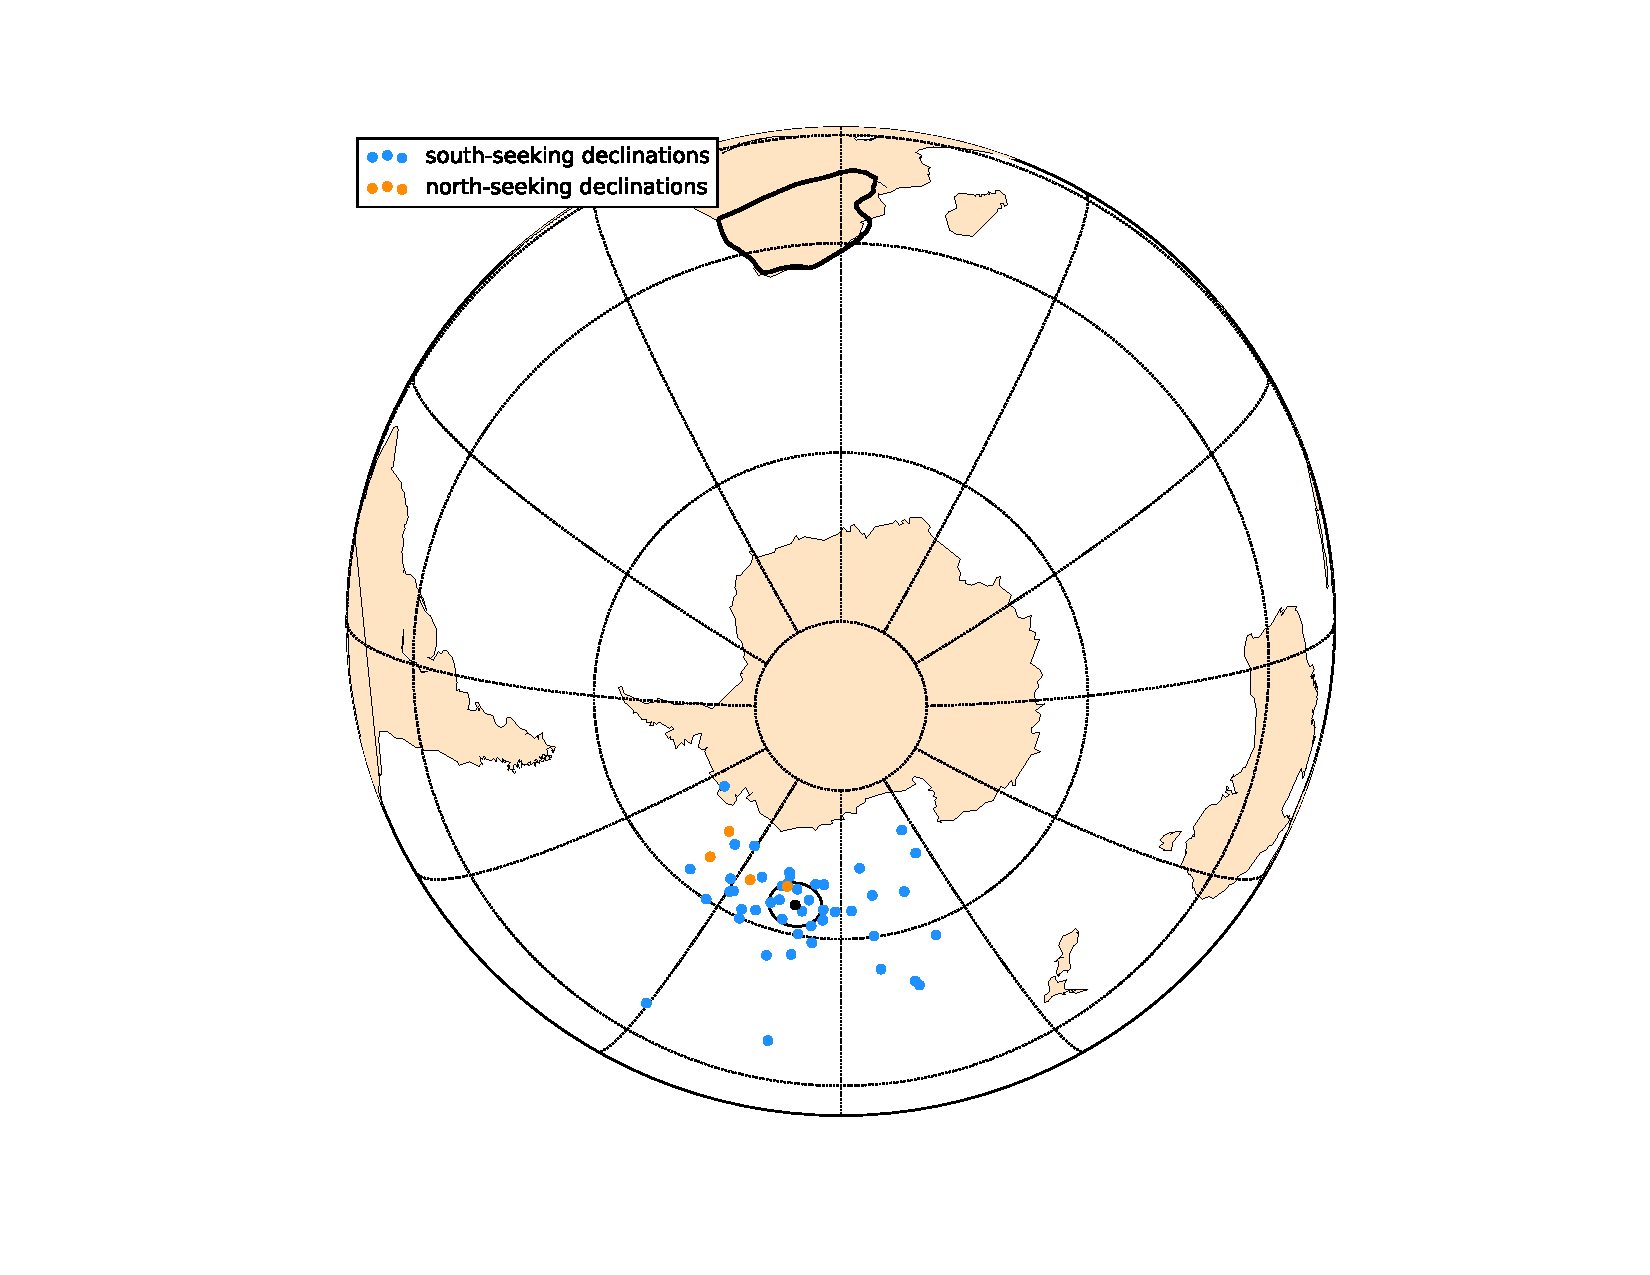
\includegraphics[width=9 cm]{figures/Umkondo_mean_pole.pdf}
\caption{\textbf{ Virtual geomagnetic poles and mean paleomagnetic pole for the Umkondo LIP.} Individual VGPs are colored orange (south-seeking polarity) and blue (north-seeking polarity). The mean pole and associated A$_{95}$ confidence ellipse are shown in black. A simplified outline of the Kalahari Craton is shown in southern Africa.}
\label{fig:pole}
\end{figure}

Paleomagnetic data have been published from intrusions and basaltic lavas of the Umkondo LIP present in the Grunehoga Province, which is a fragment of the Kalahari Craton now present in East Antarctica (Fig. \ref{fig:map}; \cite{Powell2001a,Jones2003a}). For these data to be considered with the Umkondo data, a rotation needs to be applied to restore the Grunehogna Province to Kalahari. Applying the Euler rotation (-5.3\textdegree N, 324.5\textdegree E, 58.6\textdegree CCW) suggested by \cite{Evans2009a} based on the tectonic model of \cite{Jacobs2004a} yields an overlap between the Borgmassivet pole of the Grunehogna Province \citep{Jones2003a} and the new Umkondo pole (see figure in the Supporting Information). Given that a rotation is necessary, with accompanying uncertainty, we neither use the Grunehogna data for the calculation of the mean Umkondo pole nor are these data incorporated into analyses relevant for making inferences about paleosecular variation.

\section*{Discussion}
\subsection*{Paleogeographic position of Kalahari and its relationship with Laurentia}

The resulting paleomagnetic pole for the Umkondo LIP from this study (222.1\textdegree E, 64.0\textdegree S with an A$_{95}$ of 2.6\textdegree; Table 2) has a similar position to previous poles from the province (e.g \citealt{Gose2006a}). This pole reconstructs Kalahari to an equatorial position at the time of Umkondo LIP emplacement (Fig. \ref{fig:reconstruction}). As has been established in prior work (e.g. \cite{Powell2001a, Hanson2004a}), this position is at a significant distance from Laurentia at that time with Laurentia's position at high latitudes being well-constrained by poles from the early history of Midcontinent Rift development (Fig. \ref{fig:reconstruction}; \cite{Halls1982a,Swanson-Hysell2014b}).

\begin{table}[!ht]
\small
\caption{
\textbf{Mean Umkondo LIP poles}}
\begin{tabular}{lrrrrr}
\hline
{} &    Pole\_Lat &   Pole\_Long &      A\_95 &           K &         N \\
{} &    (\textdegree N) &   (\textdegree E) & (\textdegree) &           &(sites)  \\
\hline
Umkondo Grand Mean Pole & -64.0 &  222.1 &  2.6 &   60.3 &  49 \\
Mean of north-seeking VGPs & 67.1 &   060.3 &  5.6 &  268.8 & 4 \\
Mean of south-seeking VGPs & -63.6 &  220.7 &   2.8 &   59.3 &  45 \\
\hline
\end{tabular}
\caption*{\footnotesize{Notes: These poles were calculated as the Fisher mean of VGPs from sites where the within site directional $\alpha_{95}$ was less than 15\textdegree. This filter removes 10 sites from consideration (i.e. the total number of Umkondo sites in Table 1 is 59). The north-seeking mean pole currently has too few VGPs (N=4) to be reliably used for inferences about paleogeographic change or geomagnetic field behavior between polarity intervals. The sites are from across the Kalahari craton. If a latitude/longitude of 23\textdegree S/029\textdegree E is used, the resultant calculated mean declination/inclination of the pole is: 185.7/-4.8.}}
\end{table}

It has been argued that the predominance of reversed polarity magnetizations (southeast-seeking declinations with upward inclination) within the early volcanics and intrusions of the Keweenawan Midcontinent Rift and the dominance of south-seeking declinations in the magnetization of sites from the Umkondo LIP constrains these dominant directions to the same interval of geomagnetic polarity \citep{Hanson2004a, Evans2009a}. If true, this constrains the paleopoles to be in the same hemisphere and thereby resolves the relative orientation between the continents. The interpretation that the south-seeking Umkondo directions correlate to the reversed polarity Keweenawan directions results in a relative reconstruction wherein the Grenville and Namaqua metamorphic belts, commonly interpreted to be conjugate records of a continent-continent collisional orogenic event \citep{Dalziel2000a, Jacobs2008a}, are facing away rather than towards one another (Interpretation $\#$2 in Fig. \ref{fig:reconstruction}). This relative polarity argument would be stronger if the Umkondo LIP sites were of a single magnetic polarity. However, given that four of the Umkondo sites are of north-seeking polarity, there was a geomagnetic reversal during the emplacement of the LIP. 

\begin{figure}[h!]
\begin{adjustwidth}{-0.7in}{0in}
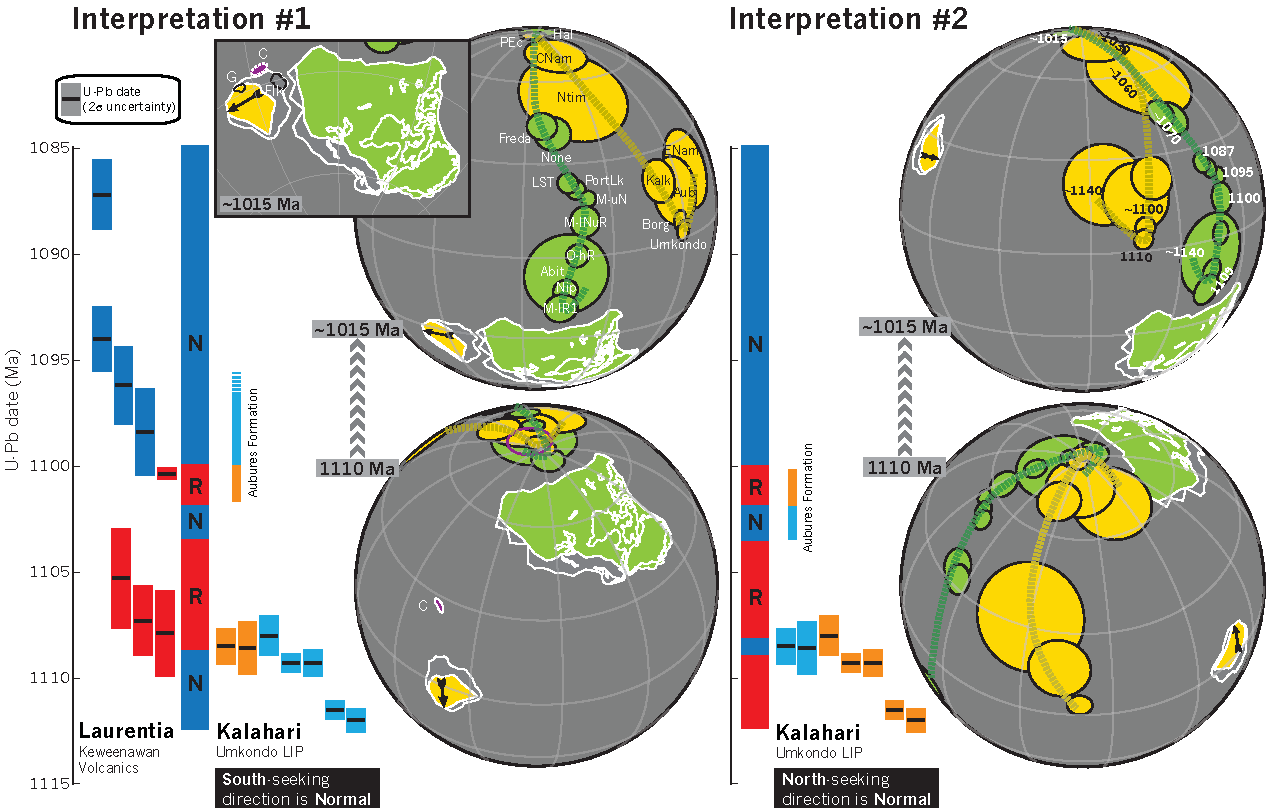
\includegraphics[width=7.9 in]{figures/reconstruction.pdf}
\end{adjustwidth}
\caption{\textbf{Paleogeography and relative geomagnetic polarity interpretations between Laurentia and Kalahari.} U--Pb dates for the Keweenawan Midcontinent Rift \citep{Davis1997a, Swanson-Hysell2014a} and the Umkondo LIP \citep{Hanson2004a} allow for two possible interpretations for the relative polarity history and paleogeographic orientation between the two Mesoproterozoic continents as described in the text. These two possibilities are illustrated at both the time of Umkondo emplacement (ca. 1110 Ma) and near the end of the Mesoproterozoic (ca. 1015 Ma) along with their apparent polar wander paths (green for Laurentia, yellow for Kalahari). Interpretation $\#$1 relates the north-seeking declinations from the Umkondo LIP with the oldest Keweenawan reversed polarity basalt flows, while interpretation $\#$2 relates those same Umkondo igneous rocks to units with normal polarity in the Keweenawan Rift. Each possibility has distinct implications for paleogeographic evolution. In contrast to interpretation $\#$2, interpretation $\#$1 allows for the continents to be reconstructed such that the Namaqua-Natal belt of Kalahari faces the Grenville margin of Laurentia and is consistent with the two continents colliding within Rodinia at ca. 1050 Ma. The position of the Coats Land (`C') and Grunehogna (`G') blocks are shown in interpretation $\#$1.}
\label{fig:reconstruction}
\end{figure}

There are seven sites in the Umkondo LIP where paleomagnetic polarity can confidently be tied to high-precision $^{207}$Pb-$^{206}$Pb baddeleyite dates given in \citep{Hanson2004a}, as shown in Table 1 and Figure \ref{fig:reconstruction} herein. Two of the Umkondo sites with north-seeking declinations have dates: the VF1/VF2 sill of South Africa with a date of 1108.6 $\pm$ 1.2 Ma and the VF4 sill of South Africa (site JM12 in Table 1) with a date of 1108.5 $\pm$ 0.8 Ma \citep{Hanson2004a}. Neither of these dates are statistically distinguishable from the Kgale Peak Sill (1108.0 $\pm$ 0.9 Ma), which has yielded both polarities, but for which we prefer a southerly declination based on our new data from sites PW1 and PW2 (Table 1; see discussion in the Supporting Information). These dates for sites with northerly declinations are statistically younger than those from two sites with southerly declinations (Timbativi Gabbro 1111.5 $\pm$ 0.4 Ma, Mokgware Sill 1112.0 $\pm$ 0.5 Ma; Fig. \ref{fig:reconstruction}; \citealt{Hanson2004a}) and apparently younger, but not at the 95$\%$ confidence level, with those from two other sites with southerly declinations (Mosolotsane 1 Sill 1109.3 $\pm$ 0.6 Ma, Shoshong Sill 1109.3 $\pm$ 0.3 Ma; recalculated from \citealt{Hanson2004a}, see Supporting Information). Taken together, these data reveal two possibilities for the geomagnetic polarity history and thereby the orientation relationship between Laurentia and Kalahari that are illustrated in Figure \ref{fig:reconstruction} and detailed below:
\begin{itemize}
\item \textbf{Interpretation $\#$1:} There was a reversal during emplacement of the Umkondo LIP from normal (southerly declinations) to reversed (northerly declinations) such that the younger sills with northerly declinations have the same polarity as the reversed polarity sites from the early magmatic stage of the Keweenawan Midcontinent Rift. This interpretation results in reconstructions wherein the Namaqua-Natal belt is oriented towards the Grenville margin of North America (interpretation $\#$1 in Fig.  \ref{fig:reconstruction}).
\item \textbf{Interpretation $\#$2:} Umkondo directions with southerly declinations represent a period of reversed geomagnetic polarity that was followed by a relatively brief interval of normal polarity represented by the northerly declinations and then a reversal back to the reversed polarity that is recorded in the early magmatic stage of the Keweenawan Midcontinent Rift. This interpretation has the dominant polarity in the Umkondo LIP correlating with the reversed polarity in the Midcontinent Rift, but with the bulk of the intrusions actually being emplaced during an earlier geomagnetic polarity interval (ca. 1112 to 1109 Ma; interpretation $\#$2 in Fig.  \ref{fig:reconstruction}). 
\end{itemize}

While it is difficult with the current data sets to definitively distinguish between these two alternatives, the subsequent apparent polar wander paths (APWP) and the polarity recorded therein provide additional context. Considering the APWP trajectory, interpretation $\#$2 effectively rules out the incorporation of Kalahari into the Rodinian supercontinent as that polarity option results in Kalahari being far-flung from Laurentia at ca. 1000 Ma (Fig. \ref{fig:reconstruction}) unless Kalahari experienced an 180\textdegree$\;$rotation (a possibility raised by \citealt{Jacobs2008a}). While this exclusion of Kalahari from Rodinia is possible, there are data that support the collision of Kalahari with Laurentia within the supercontinent including the hypothesized transfer of the Coats Land Block \citep{Loewy2011a}. The Coats Land Block is inferred to have been part of Laurentia through the similarity of Pb isotopic data between Keweenawan rift volcanics and the Coats Land nunatuks \citep{Loewy2011a} which have been dated between 1113 and 1106 Ma \citep{Gose1997a}. We note, however, that reconstruction of Coats Land using the pole of \cite{Gose1997a} results in a position of Coats Land offshore of Laurentia unless the pole is correlated to younger (ca. 1095 to 1085 Ma) rather than contemporaneous (ca. 1105 Ma) Keweenawan Rift poles. A reconstruction using the \cite{Gose1997a} pole results in a position of Coats Land in the gap between Laurentia and Kalahari (Fig. \ref{fig:reconstruction}). This position is intriguing given that it allows Coats Land to be an accreted terrane to either Kalahari (as argued by \cite{Dalziel2000a}) or to Laurentia that then left with Kalahari when the cratons rifted apart. An interpretation wherein Coats Land was originally of Laurentian affinity or became sutured between Laurentia and Kalahari favors the reconstruction shown as interpretation $\#$1 (Fig. \ref{fig:reconstruction}).

Another line of evidence comes from the dominant south-seeking declinations of the Aubures Formation sedimentary rocks that post-date the Umkondo LIP \citep{Kasbohm2015a}. The lowermost portion of those sedimentary rocks (which contain detrital zircons of Umkondo LIP age) have north-directed declinations while the subsequent majority of the formation appears to solely have south-directed declinations \citep{Kasbohm2015a}. As argued by \cite{Kasbohm2015a}, it is likely that these sediments were deposited during the interval from 1100 Ma to at least 1086 Ma during which the Keweenawan Midcontinent Rift appears to be solely normal polarity \citep{Swanson-Hysell2014a}. This correlation favors interpretation $\#$1 above (Fig. \ref{fig:reconstruction}) where the south-seeking Umkondo declinations correspond to normal polarity in Laurentia. It is possible that the Aubores sediments were all deposited prior to 1100 Ma and have the opposite polarity interpretation as illustrated in interpretation $\#$1 above (Fig. \ref{fig:reconstruction}). Overall, these data favor the model in which the Namaqua-Natal belt can be interpreted as a conjugate to the Grenville margin, and therefore Kalahari could have been conjoined with Laurentia by the end of the Mesoproterozoic. These models can be tested by further refining the geomagnetic polarity histories of Laurentia and Kalahari with future high-precision geochronology that is robustly paired with paleomagnetic data. 

\subsection*{Paleosecular variation}

With VGPs separated out at the cooling unit (site) level, we are able to analyze the distribution of the VGPs to make inferences about paleosecular variation of the geomagnetic field. Existing U-Pb dates from the Umkondo LIP are quite close together in age implying the the province was emplaced rapidly (within ca. 3 million years) as is the case for some other well-constrained intraplate large magmatic events such as the Central Atlantic Magmatic Province \citep{Blackburn2013a} and the Karoo-Ferrar Province \citep{Sell2014a, Burgess2015a}. Notably, this magmatic history contrasts with the evidence for prolonged magmatic activity in the Keweenawan Midcontinent Rift wherein applications of paleosecular variation analyses need to be cognizant of the evidence for progressive directional change that is associated with rapid plate motion rather than secular variation \citep{Davis1997a, Swanson-Hysell2009a, Swanson-Hysell2014a}. Given the evidence for rapid emplacement of the Umkondo LIP, we interpret the variation of VGP positions (Fig. \ref{fig:pole}) as dominantly arising from secular variation without significant apparent or true polar wander. 

The calculated value of VGP scatter (S) utilizing a within site correction (see \cite{Biggin2008b}) is 10.1. This value is lower than the value of 13.0 recently reported by \cite{Veikkolainen2014b}, which was based on 27 sites taken from \cite{Gose2006a} and lower still from the value of 14.2 reported by \cite{Smirnov2011b} calculated from 15 sites. This adjustment brings the S value for the Umkondo Province in better alignment with the trend of values as observed in other Proterozoic data and as predicted by a Model G fit to compiled data from 1.0 to 2.2 Ga \citep{Smirnov2011b,Veikkolainen2014b}. One caveat is that intrusive units lacking radiometric dates are in many cases assigned to a given igneous province based on their directions of magnetization. If a particular intrusion has a significantly different direction due to paleosecular variation, it could be erroneously excluded from the VGP database for that igneous province, thereby biasing the paleosecular variation analysis and reducing the value calculated for S. This potential for bias is present with our methodology in dealing with the Umkondo data as well as for many other studies focused on igneous intrusive units, particularly for the Precambrian, given the spatial overlap between multiple igneous provinces and the paucity of radiometric dates. \cite{Deenen2011a} demonstrated how the application of filters on random draws from paleosecular variation models (such as excluding VGPS $>$45\textdegree$\;$from the mean) can significantly skew estimates for VGP scatter (S) given how strongly the parameter is affected by outliers. The skewing of VGP scatter estimates by outliers has long been considered and led to the proposal by \cite{Vandamme1994a} to use a recursive approach to prune data sets with a variable cutoff filter. However, as shown by \cite{Smirnov2011b}, compilations of ancient cooling unit VGPs reveal data with low scatter that are relatively unaffected by fixed cutoffs or by the Vandamme variable cutoff. While this low scatter could be reflective of a more strongly dipolar field (as argued by \citealt{Smirnov2011b}) it could also be biased by the procedures used to group intrusions, particularly in ancient cratons cross-cut by multiple igneous provinces. Estimates for the elongation parameter used to described the ellipticity of a distribution are also affected by the outliers which may be preferentially excluded in such compilations, but are less sensitive to their presence as shown by \cite{Deenen2011a}. Details of the elongation parameter and the estimate for it obtained using the Umkondo data are described below. 

As discussed in \cite{Tauxe2004a}, the eigenvalues of the orientation matrix of the distribution of mean directions from paleomagnetic sites can be used to calculate the elongation parameter (E) as the ratio of $\tau_2$/$\tau_3$. Statistical secular variation models predict a relationship wherein elongation is higher at lower inclination (\cite{Tauxe2008a}; Fig. \ref{fig:EI}). It is preferable to have as many unique readings for the field as possible to determine elongation \citep{Tauxe2008a}. According to our compilation, 49 VGPs are available for this analysis (applying the $\alpha_{95}<15$\textdegree$\;$filter) and hopefully more can be added in the future to make the estimate more robust. The uncertainty of the elongation determination using the current dataset can be estimated through a bootstrap method as described in \cite{Tauxe2008a}. Through this analysis, we find an elongation value of 2.7 that corresponds with the predicted elongation/inclination behavior of the TK03.GAD model, developed by Tauxe and Kent (2004) to represent the secular variation of a time-averaged geocentric axial dipole (GAD) field, with the caveat that the 95$\%$ bootstrapped confidence bounds are large, as they are for data from the other LIPs that are compiled in Fig. \ref{fig:EI}. We also recalculate the elongation value for data developed by \cite{Tauxe2009a} from the ca. 1095 Ma North Shore Volcanic Group (NSVG) of the Keweenawan Midcontinent Rift. Data from the upper NSVG alone, excluding units from the overlying Schroeder-Lutsen Basalts and the lower reversed portion of the group, results in an elongation value of 1.7 (Fig. \ref{fig:EI}; see the Supporting Information for details). This slightly modified elongation estimate is also close to that predicted by the TK03.GAD as was presented by \cite{Tauxe2009a}. The similarity in age between the Umkondo and NSVG igneous units combined with their quite distinct inclinations makes this comparison well-suited for testing of the TK03.GAD model and is consistent with a dominantly dipolar field in the late Mesoproterozoic quantitatively similar to the field in more recent time. This result adds additional support to the conclusion of \cite{Tauxe2009a} that the elongation and inclination trend predicted by the TK03.GAD paleosecular variation model that was developed for the recent field is robust further back in Earth history. However, the large 95 per cent confidence bounds on the elongation values introduces considerable uncertainty when comparing these data to model predictions (Fig. 5). Also, while some non-dipole contributions can lead to distinct elongation-inclination trends (e.g. a 20 per cent axial octupole; Tauxe and Kodama, 2009), others have similar elongation-inclination relationships to that predicted for a 100 per cent GAD field (e.g. a 5 per cent axial quadrupole; Tauxe et al., 2008). The assumption that this elongation vs. inclination trend holds throughout time is an integral component of the E/I method for correction for inclination flattening in sedimentary rocks (see \citealt{Tauxe2008a}) which highlights the importance of continuing to develop and compile large datasets from many sites. Efforts both to increase the number of sites from the LIPs currently within the compilation shown in Figure \ref{fig:EI} and to compile and develop data from additional igneous provinces can further test the robustness of this E/I relationship through time. The compilation of VGPs for the Umkondo Province developed here at the cooling unit level provides a framework for revision and addition. Further additions can extend the robustness of estimates of elongation and other parameters.

\begin{figure}[h!]
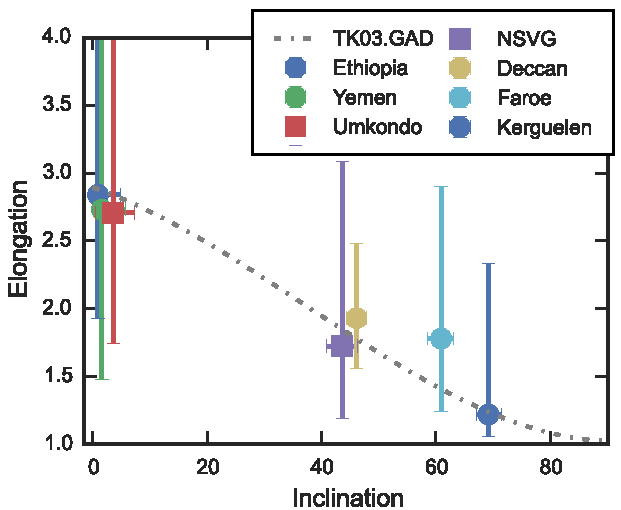
\includegraphics[width=9 cm]{figures/EI_revised.pdf}
\caption{\textbf{ Elongation vs. inclination for Umkondo and other LIPs shown with the curve as predicted by the TK03.GAD model.} Elongation and inclination values are shown with their bootstrapped 95$\%$ confidence bounds (see Supporting Information and \cite{Tauxe2008a} for details on data sets and calculations).}
\label{fig:EI}
\end{figure}

\section*{Conclusions}

Through the acquisition of new data from sills in Botswana and the careful compilation of previously published data, we have developed a new grand mean paleomagnetic pole for the ca. 1112-1108 Ma Umkondo large igneous province. The relative ages of the two polarities recorded in Umkondo igneous units as constrained by U-Pb dates and consideration of the subsequent apparent polar wander path of Kalahari leads us to favor a model wherein southerly directions in the Umkondo Province correspond with normal geomagnetic polarity in the Keweenawan Midcontinent Rift of Laurentia. In contrast to equating these directions with reversed polarity, this interpretation ($\#$1) has the Namaqua-Natal belt of Kalahari facing towards the Grenville Belt of Laurentia and allows for the two continents to have become subsequently conjoined within Rodinia. This model can be further tested through the development of new high precision radiometric age constraints that are well-paired with paleomagnetic data. The compilation of VGPs at the site (cooling unit) level, allows for their distribution to be interpreted in terms of paleosecular variation. We argue that estimates of scatter have a high potential to be biased to low values since magnetization directions themselves are commonly used to determine whether igneous intrusions belong in certain provinces. As a result, directions at appreciable angles to the mean rarely make it into compilations used for paleosecular variation analyses based on the directions of intrusions. Estimates of elongation can also be biased by the inherent exclusion of seemingly disparate points in such datasets, but to a lesser extent. In the case of the Umkondo data, the elongation estimate is consistent with that predicted by the TK03.GAD model. This consistency extends to the elongation estimate for the slightly younger volcanics of the upper North Shore Volcanic Group (ca. 1095 Ma). Taken together, these data are consistent with a dominantly dipolar field in the late Mesoproterozoic. 

\section*{Acknowledgments}
This research was supported by the National Science Foundation under grants EAR-PF 1045635 and EAR-1419894 awarded to Swanson-Hysell. Additional support came from the Institute for Rock Magnetism, Texas Christian University and the Botswana Geological Survey. We are grateful to the Botswana Ministry of Minerals, Energy and Water Resources for granting us a permit to conduct research in Botswana and to Brets Direng of the Botswana Geological Survey for advice and important logistical support. Gwandu Kewame, Gaune Motsoela and Othogile Rulele of the Botswana Geological Survey assisted with field work. Kristofer Asp helped with sample preparation. Discussions with David Evans and reviews by Lauri Pesonen and Michel de Kock improved the manuscript. 

\singlespacing

\begin{thebibliography}{49}
\expandafter\ifx\csname natexlab\endcsname\relax\def\natexlab#1{#1}\fi

\bibitem[Biggin et~al.(2008)Biggin, van Hinsbergen, Langereis, Straathof, \&
  Deenen]{Biggin2008b}
Biggin, A.~J., van Hinsbergen, D. J.~J., Langereis, C.~G., Straathof, G.~B., \&
  Deenen, M. H.~L., 2008.
\newblock {Geomagnetic secular variation in the Cretaceous Normal Superchron
  and in the Jurassic}, {\it Physics of the Earth and Planetary Interiors\/},
  {\bf 169}(1--4), 3--19.

\bibitem[Blackburn et~al.(2013)Blackburn, Olsen, Bowring, McLean, Kent, Puffer,
  McHone, Rasbury, \& Et-Touhami]{Blackburn2013a}
Blackburn, T.~J., Olsen, P.~E., Bowring, S.~A., McLean, N.~M., Kent, D.~V.,
  Puffer, J., McHone, G., Rasbury, E.~T., \& Et-Touhami, M., 2013.
\newblock Zircon {U-Pb} geochronology links the end-{T}riassic extinction with
  the {Central Atlantic Magmatic Province}, {\it Science\/}, {\bf 340},
  941--945.

\bibitem[Brandl(1981)]{Brandl1981a}
Brandl, G., 1981.
\newblock Geological map of the {M}essina area (sheet 2230), {\it South Africa
  Geological Survey, Pretoria, 1:250,000 scale\/}.

\bibitem[Brandl(1985)]{Brandl1985a}
Brandl, G., 1985.
\newblock Geological map of the {P}ietersburg area (sheet 2328), {\it South
  Africa Geological Survey, Pretoria, 1:250,000 scale\/}.

\bibitem[Burgess et~al.(2015)Burgess, Bowring, Fleming, \&
  Elliot]{Burgess2015a}
Burgess, S.~D., Bowring, S.~A., Fleming, T.~H., \& Elliot, D.~H., 2015.
\newblock {High-precision geochronology links the Ferrar large igneous province
  with early-Jurassic ocean anoxia and biotic crisis}, {\it Earth and Planetary
  Science Letters\/}, {\bf 415}, 90--99.

\bibitem[Carney et~al.(1994)Carney, Aldiss, \& Lock]{Carney1994a}
Carney, J., Aldiss, D., \& Lock, N., 1994.
\newblock The geology of {B}otswana, {\it Botswana Geological Survey
  Bulletin\/}, {\bf 37}.

\bibitem[Dalziel et~al.(2000)Dalziel, Mosher, \& Gahagan]{Dalziel2000a}
Dalziel, I. W.~D., Mosher, S., \& Gahagan, L.~M., 2000.
\newblock Laurentia--{K}alahari collision and the assembly of {R}odinia, {\it
  The Journal of Geology\/}, {\bf 108}(5), 499--513.

\bibitem[Davis \& Green(1997)]{Davis1997a}
Davis, D. \& Green, J., 1997.
\newblock Geochronology of the {N}orth {A}merican {M}idcontinent rift in
  western {L}ake {S}uperior and implications for its geodynamic evolution, {\it
  Canadian Journal of Earth Science\/}, {\bf 34}, 476--488.

\bibitem[de~Kock et~al.(2014)de~Kock, Ernst, S{\"o}derlund, Jourdan, Hofmann,
  Le~Gall, Bertrand, Chisonga, Beukes, Rajesh, Moseki, \& Fuchs]{Kock2014a}
de~Kock, M.~O., Ernst, R., S{\"o}derlund, U., Jourdan, F., Hofmann, A.,
  Le~Gall, B., Bertrand, H., Chisonga, B.~C., Beukes, N., Rajesh, H.~M.,
  Moseki, L.~M., \& Fuchs, R., 2014.
\newblock {Dykes of the 1.11 Ga Umkondo LIP, Southern Africa: Clues to a
  complex plumbing system}, {\it Precambrian Research\/}, {\bf 249}, 129--143.

\bibitem[Deenen et~al.(2011)Deenen, Langereis, van Hinsbergen, \&
  Biggin]{Deenen2011a}
Deenen, M. H.~L., Langereis, C.~G., van Hinsbergen, D. J.~J., \& Biggin, A.~J.,
  2011.
\newblock Geomagnetic secular variation and the statistics of palaeomagnetic
  directions, {\it Geophysical Journal International\/}.

\bibitem[Evans(2009)]{Evans2009a}
Evans, D., 2009.
\newblock The palaeomagnetically viable, long-lived and all-inclusive {R}odinia
  supercontinent reconstruction, in {\em Ancient Orogens and Modern
  Analogues\/}, vol. 327, pp. 371--404, eds Murphy, J., Keppie, J., \& Hynes,
  A., Geological Society of London Special Publication.

\bibitem[Feinberg et~al.(2015)Feinberg, Solheid, Swanson-Hysell, Jackson, \&
  Bowles]{Feinberg2015a}
Feinberg, J., Solheid, P., Swanson-Hysell, N., Jackson, M., \& Bowles, J.,
  2015.
\newblock Full vector low-temperature magnetic measurements of geologic
  materials, {\it Geochemistry, Geophysics, Geosystems\/}, {\bf 16}, 301--314.

\bibitem[Geng et~al.(2014)Geng, Brandl, Sun, Wong, \& Kr{\"o}ner]{Geng2014a}
Geng, H., Brandl, G., Sun, M., Wong, J., \& Kr{\"o}ner, A., 2014.
\newblock Zircon ages defining deposition of the palaeoproterozoic soutpansberg
  group and further evidence for eoarchaean crust in south africa, {\it
  Precambrian Research\/}, {\bf 249}(0), 247 -- 262.

\bibitem[Gose et~al.(1997)Gose, Helper, Connelly, Hutson, \&
  Dalziel]{Gose1997a}
Gose, W., Helper, M., Connelly, J., Hutson, F., \& Dalziel, I., 1997.
\newblock Paleomagnetic data and {U-Pb} isotopic age determinations from
  {C}oats {L}and, {A}ntarctica: {I}mplications for late {P}roterozoic plate
  reconstructions, {\it Journal of Geophysical Research\/}, {\bf 102}(B4),
  7887--7902.

\bibitem[Gose et~al.(2006)Gose, Hanson, Dalziel, Pancake, \& Seidel]{Gose2006a}
Gose, W.~A., Hanson, R.~E., Dalziel, I. W.~D., Pancake, J.~A., \& Seidel,
  E.~K., 2006.
\newblock Paleomagnetism of the {1.1 Ga Umkondo large igneous province in
  southern Africa}, {\it J. Geophys. Res.\/}, {\bf 111}(B9),
  10.1029/2005JB003897.

\bibitem[Halls \& Pesonen(1982)]{Halls1982a}
Halls, H. \& Pesonen, L., 1982.
\newblock Paleomagnetism of {K}eweenawan rocks, {\it Geological Society of
  America Memoirs\/}, {\bf 156}, 173--201.

\bibitem[Hanson et~al.(2004{\natexlab{a}})Hanson, Crowley, Bowring, Ramezani,
  Gose, Dalziel, Pancake, Seidel, Blenkinsop, \& Mukwakwami]{Hanson2004a}
Hanson, R., Crowley, J., Bowring, S., Ramezani, J., Gose, W., Dalziel, I.,
  Pancake, J., Seidel, E., Blenkinsop, T., \& Mukwakwami, J.,
  2004{\natexlab{a}}.
\newblock Coeval large-scale magmatism in the {K}alahari and {L}aurentian
  {C}ratons during {R}odinia assembly, {\it Science\/}, {\bf 304}, 1126--1129.

\bibitem[Hanson et~al.(2004{\natexlab{b}})Hanson, Gose, Crowley, Ramezani,
  Bowring, Bullen, Hall, Pancake, \& Mukwakwami]{Hanson2004b}
Hanson, R., Gose, W., Crowley, J., Ramezani, J., Bowring, S., Bullen, D., Hall,
  R., Pancake, J., \& Mukwakwami, J., 2004{\natexlab{b}}.
\newblock Paleoproterozoic intraplate magmatism and basin development on the
  {K}aapvaal {C}raton: Age, paleomagnetism and geochemistry of $\sim$1.93 to
  $\sim$1.87 ga post-{W}aterberg dolerites, {\it South African Journal of
  Geology\/}, {\bf 107}(1-2), 233--254.

\bibitem[Hanson et~al.(2006)Hanson, Harmer, Blenkinsop, Bullen, Dalziel, Gose,
  Hall, Kampunzu, Key, Mukwakwami, Munyanyiwa, Pancake, Seidel, \&
  Ward]{Hanson2006a}
Hanson, R.~E., Harmer, R.~E., Blenkinsop, T.~G., Bullen, D.~S., Dalziel, I.
  W.~D., Gose, W.~A., Hall, R.~P., Kampunzu, A.~B., Key, R.~M., Mukwakwami, J.,
  Munyanyiwa, H., Pancake, J.~A., Seidel, E.~K., \& Ward, S.~E., 2006.
\newblock {Mesoproterozoic intraplate magmatism in the Kalahari Craton: A
  review}, {\it Journal of African Earth Sciences\/}, {\bf 46}(1-2), 141--167.

\bibitem[Hanson et~al.(2011)Hanson, Rioux, Gose, Blackburn, Bowring,
  Mukwakwami, \& Jones]{Hanson2011b}
Hanson, R.~E., Rioux, M., Gose, W.~A., Blackburn, T.~J., Bowring, S.~A.,
  Mukwakwami, J., \& Jones, D.~L., 2011.
\newblock {Paleomagnetic and geochronological evidence for large-scale
  post--1.88 Ga displacement between the Zimbabwe and Kaapvaal cratons along
  the Limpopo belt}, {\it Geology\/}, {\bf 39}(5), 487--490.

\bibitem[Jacobs \& Thomas(2004)]{Jacobs2004a}
Jacobs, J. \& Thomas, R.~J., 2004.
\newblock Himalayan-type indenter-escape tectonics model for the southern part
  of the late {Neoproterozoic--early Paleozoic East African--Antarctic orogen},
  {\it Geology\/}, {\bf 32}(8), 721--724.

\bibitem[Jacobs et~al.(2008)Jacobs, Pisarevsky, Thomas, \& Becker]{Jacobs2008a}
Jacobs, J., Pisarevsky, S., Thomas, R.~J., \& Becker, T., 2008.
\newblock {The Kalahari Craton during the assembly and dispersal of Rodinia},
  {\it Precambrian Research\/}, {\bf 160}(1-2), 142--158.

\bibitem[Jones \& McElhinny(1966)]{Jones1966a}
Jones, D. \& McElhinny, M., 1966.
\newblock Paleomagnetic correlation of basic intrusions in the {P}recambrian of
  southern {A}frica, {\it Journal of Geophysical Research\/}, {\bf 71}(2),
  543--552.

\bibitem[Jones et~al.(2003)Jones, Bates, Li, Corner, \& Hodgkinson]{Jones2003a}
Jones, D., Bates, M., Li, Z., Corner, B., \& Hodgkinson, G., 2003.
\newblock Paleomagnetic results from the ca. 1130 {M}a {B}orgmassivet
  intrusions in the {A}hlmannryggen region of {D}ronning {M}aud {L}and,
  {A}ntarctica, and tectonic implications, {\it Tectonophysics\/}, {\bf 375},
  247--260.

\bibitem[Kasbohm et~al.(2015)Kasbohm, Evans, Panzik, Hofmann, \&
  Linneman]{Kasbohm2015a}
Kasbohm, J., Evans, D., Panzik, J.~E., Hofmann, M., \& Linneman, U., 2015.
\newblock {Paleomagnetic and geochronological data from the late Mesproterozoic
  redbed sedimentary rocks on the western margin of Kalahari craton}, in {\em
  Supercontinent Cycles Through Earth History\/}, vol. 424, eds Li, Z.~X.,
  Evans, D. A.~D., \& Murphy, J.~B., Geological Society, London, Special
  Publications.

\bibitem[Kirschvink(1980)]{Kirschvink1980a}
Kirschvink, J., 1980.
\newblock The least-squares line and plane and the analysis of paleomagnetic
  data, {\it Geophysical Journal of the Royal Astronomical Society\/}, {\bf
  62}(3), 699--718.

\bibitem[Li et~al.(2008)]{Li2008a}
Li, Z.~X. et~al., 2008.
\newblock Assembly, configuration, and break-up history of {R}odinia: A
  synthesis, {\it Precambrian Research\/}, {\bf 160}(1-2), 179--210.

\bibitem[Loewy et~al.(2011)Loewy, Dalziel, Pisarevsky, Connelly, Tait, Hanson,
  \& Bullen]{Loewy2011a}
Loewy, S.~L., Dalziel, I. W.~D., Pisarevsky, S., Connelly, J.~N., Tait, J.,
  Hanson, R.~E., \& Bullen, D., 2011.
\newblock {Coats Land crustal block, East Antarctica: A tectonic tracer for
  Laurentia?}, {\it Geology\/}.

\bibitem[Mc{E}lhinny(1966)]{McElhinny1966a}
Mc{E}lhinny, M., 1966.
\newblock The paleomagnetism of {U}mkondo lavas, eastern southern {R}hodesia,
  {\it Geophysical Journal of the Royal Astronomical Society\/}, {\bf 10}(4),
  375--381.

\bibitem[Mc{E}lhinny \& Opdyke(1964)]{McElhinny1964b}
Mc{E}lhinny, M. \& Opdyke, N., 1964.
\newblock The paleomagnetism of the {P}recambrian dolerites of eastern
  {S}outhern {R}hodesia, an example of geologic correlation by rock magnetism,
  {\it Journal of Geophysical Research\/}, {\bf 69}(12), 2465--2475.
  
\bibitem[Mc{F}adden \& Mc{E}lhinny(1990)]{McFadden1990a}
Mc{F}adden, P. \& Mc{E}lhinny, M., 1990.
\newblock Classification of the reversal test in palaeomagnetism, {\it
  Geophysical Journal International\/}, {\bf 103}, 725--729.

\bibitem[Moabi et~al.(2015)Moabi, Grantham, Roberts, Roux, \&
  Matola]{Moabi2015a}
Moabi, N.~G., Grantham, G.~H., Roberts, J., Roux, P.~l., \& Matola, R., 2015.
\newblock {The geology and geochemistry of the Espungabera Formation of central
  Mozambique and its tectonic setting on the eastern margin of the Kalahari
  Craton}, {\it Journal of African Earth Sciences\/}, {\bf 101}(0), 96--112.

\bibitem[Modie(1996)]{Modie1996a}
Modie, B. N.~J., 1996.
\newblock {Depositional environments of the Meso- to Neoproterozoic
  Ghanzi-Chobe belt, northwest Botswana}, {\it Journal of African Earth
  Sciences\/}, {\bf 22}(3), 255--268.

\bibitem[Pancake(2001)]{Pancake2001a}
Pancake, J., 2001.
\newblock {\it Geochronological and paleomagnetic studies of Mesoproterozoic
  mafic igneous rocks in Botswana\/}, Master's thesis, Texas Christian
  University.

\bibitem[Powell et~al.(2001)Powell, Jones, Pisarevsky, \& Wingate]{Powell2001a}
Powell, C., Jones, D., Pisarevsky, S., \& Wingate, M., 2001.
\newblock Paleomagnetic constraints on the position of the {K}alahari craton in
  {R}odinia, {\it Precambrian Research\/}, {\bf 110}, 33--46.

\bibitem[Seidel(2004)]{Seidel2004a}
Seidel, E., 2004.
\newblock {\it Paleomagnetic and geochronological study of parts of the 1.1
  {G}a {U}mkondo igneous province in {S}outh {A}frica\/}, Ph.D. thesis, Texas
  Christian University.

\bibitem[Sell et~al.(2014)Sell, Ovtcharova, Guex, Bartolini, Jourdan,
  Spangenberg, Vicente, \& Schaltegger]{Sell2014a}
Sell, B., Ovtcharova, M., Guex, J., Bartolini, A., Jourdan, F., Spangenberg,
  J.~E., Vicente, J.-C., \& Schaltegger, U., 2014.
\newblock {Evaluating the temporal link between the Karoo LIP and
  climatic--biologic events of the Toarcian Stage with high-precision U--Pb
  geochronology}, {\it Earth and Planetary Science Letters\/}, {\bf 408}(0), 48
  -- 56.

\bibitem[Smirnov et~al.(2011)Smirnov, Tarduno, \& Evans]{Smirnov2011b}
Smirnov, A.~V., Tarduno, J.~A., \& Evans, D. A.~D., 2011.
\newblock Evolving core conditions ca. 2 billion years ago detected by
  paleosecular variation, {\it Physics of the Earth and Planetary Interiors\/},
  {\bf 187}, 225--231.

\bibitem[S{\"o}derlund et~al.(2010)S{\"o}derlund, Hofmann, Klausen, Olsson,
  Ernst, \& Persson]{Soderlund2010a}
S{\"o}derlund, U., Hofmann, A., Klausen, M.~B., Olsson, J.~R., Ernst, R.~E., \&
  Persson, P.-O., 2010.
\newblock Towards a complete magmatic barcode for the {Z}imbabwe craton:
  Baddeleyite {U--Pb} dating of regional dolerite dyke swarms and sill
  complexes, {\it Precambrian Research\/}, {\bf 183}(3), 388--398.

\bibitem[Svensen et~al.(2012)Svensen, Corfu, Polteau, Hammer, \&
  Planke]{Svensen2012a}
Svensen, H., Corfu, F., Polteau, S., Hammer, {\O}., \& Planke, S., 2012.
\newblock {Rapid magma emplacement in the Karoo Large Igneous Province}, {\it
  Earth and Planetary Science Letters\/}, {\bf 325--326}(0), 1--9.

\bibitem[Swanson-Hysell et~al.(2009)Swanson-Hysell, Maloof, Weiss, \&
  Evans]{Swanson-Hysell2009a}
Swanson-Hysell, N.~L., Maloof, A.~C., Weiss, B.~P., \& Evans, D. A.~D., 2009.
\newblock No asymmetry in geomagnetic reversals recorded by
  1.1-billion-year-old {K}eweenawan basalts, {\it Nature Geoscience\/}, {\bf
  2}, 713--717.

\bibitem[Swanson-Hysell et~al.(2014{\natexlab{a}})Swanson-Hysell, Burgess,
  Maloof, \& Bowring]{Swanson-Hysell2014a}
Swanson-Hysell, N.~L., Burgess, S.~D., Maloof, A.~C., \& Bowring, S.~A.,
  2014{\natexlab{a}}.
\newblock Magmatic activity and plate motion during the latent stage of
  {M}idcontinent {R}ift development, {\it Geology\/}, {\bf 42}, 475--478.

\bibitem[Swanson-Hysell et~al.(2014{\natexlab{b}})Swanson-Hysell, Vaughan,
  Mustain, \& Asp]{Swanson-Hysell2014b}
Swanson-Hysell, N.~L., Vaughan, A.~A., Mustain, M.~R., \& Asp, K.~E.,
  2014{\natexlab{b}}.
\newblock {Confirmation of progressive plate motion during the Midcontinent
  Rift's early magmatic stage from the Osler Volcanic Group, Ontario, Canada},
  {\it Geochemistry Geophysics Geosystems\/}, {\bf 15}, 2039--2047.

\bibitem[Swift(1962)]{Swift1962a}
Swift, W.~H., 1962.
\newblock {The geology of the Middle Sabi Valley}, {\it Southern Rhodesia
  Geological Survey Bulletin\/}, {\bf 52}.

\bibitem[Tauxe \& Kent(2004)]{Tauxe2004a}
Tauxe, L. \& Kent, D., 2004.
\newblock A simplified statistical model for the geomagnetic field and the
  detection of shallow bias in paleomagnetic inclinations: was the ancient
  magnetic field dipolar?, in {\em Timescales of the paleomagnetic field\/},
  vol. 145 of {\bf Geophysical Monograph}, pp. 101--116, eds Channell, J.,
  Kent, D., Lowrie, W., \& Meert, J., American Geophysical Union.

\bibitem[Tauxe \& Kodama(2009)]{Tauxe2009a}
Tauxe, L. \& Kodama, K., 2009.
\newblock Paleosecular variation models for ancient times: Clues from
  {K}eweenawan lava flows, {\it Physics of the Earth and Planetary
  Interiors\/}, {\bf 177}, 31--45.

\bibitem[Tauxe et~al.(2008)Tauxe, Kodama, \& Kent]{Tauxe2008a}
Tauxe, L., Kodama, K., \& Kent, D., 2008.
\newblock Testing corrections for paleomagnetic inclination error in
  sedimentary rocks: A comparative approach, {\it Physics of the Earth and
  Planetary Interiors\/}, {\bf 169}(1-4), 152--165.

\bibitem[Vandamme(1994)]{Vandamme1994a}
Vandamme, D., 1994.
\newblock A new method to determine paleosecular variation, {\it Physics of the
  Earth and Planetary Interiors\/}, {\bf 85}(1--2), 131--142.

\bibitem[Veikkolainen \& Pesonen(2014)]{Veikkolainen2014b}
Veikkolainen, T. \& Pesonen, L.~J., 2014.
\newblock Palaeosecular variation, field reversals and the stability of the
  geodynamo in the {P}recambrian, {\it Geophysical Journal International\/},
  {\bf 199}(3), 1515--1526.

\bibitem[Verwey(1939)]{Verwey1939a}
Verwey, E. J.~W., 1939.
\newblock Electronic conduction of magnetite ({F}e$_3${O}$_4$) and its
  transition point at low temperatures, {\it Nature\/}, {\bf 144}, 327--328.
  
\bibitem[Watson(1956)]{Watson1956a}
Watson, G., 1956.
\newblock A test for randomness of directions, {\it Geophysical Journal
  International\/}, {\bf 7}, 160--161.

\end{thebibliography}


%\bibliographystyle{gji}
%\bibliography{allrefs}

\end{document}

